\providecommand{\main}{../../..}
\documentclass[\main/main.tex]{subfiles}
\begin{document}

\subsection{Esercizio 10}
Un centro sociale cerca una nuova sede: esistono quattro alternative $(A, B, C, D)$ oltre all'alternativa $0$ (restare nella sede attuale). Si è stabilito che la scelta tra le cinque alternative debba essere definitiva e che sarà fatta in base a tre fattori: costi, accessibilità e prestigio. E fornita una tabella indicante le utilità per ciascuna alternativa e fattore in una scala tra $0$ e $100$. E fornito anche un vettore di pesi dei tre fattori.

\begin{table}
  \begin{tabular}{c|LLLLL}
    Indicatori    & A  & B  & C  & D   & 0   \\
    \hline
    Costi         & 90 & 90 & 90 & 1   & 100 \\
    Accessibilità & 12 & 13 & 10 & 100 & 37  \\
    Prestigio     & 30 & 1  & 5  & 100 & 10  \\
  \end{tabular}
  \begin{tabular}{c|c}
           & Pesi           \\
    \hline
    $\w_1$ & $\sfrac{1}{3}$ \\
    $\w_2$ & $\sfrac{1}{3}$ \\
    $\w_3$ & $\sfrac{1}{3}$ \\
  \end{tabular}
\end{table}

\begin{enumerate}
  \item Si ordinino le alternative in base ai pesi assegnati.
  \item Si faccia un'analisi di sensitività rispetto al peso dei costi, per stabilire l'intervallo di pesi in cui l'alternativa scelta resta la migliore.
  \item Si rappresentino nello spazio dei pesi i supporti delle diverse alternative.
\end{enumerate}

\subsection{Soluzione esercizio 10}
\begin{table}
  \begin{tabular}{c|LLLLL}
            & A  & B     & C  & D  & 0  \\
    \hline
    Utilità & 44 & 34.66 & 35 & 67 & 49
  \end{tabular}
\end{table}

In ordine le alternative risultano essere: $D, 0, A, C, B$.

Assegnando $\w_1 = 1 - \w_2 - \w_3$ e $\w_2 + \w_3 \leq 1$ si può rappresentare lo spazio dei supporti come:

\begin{figure}
  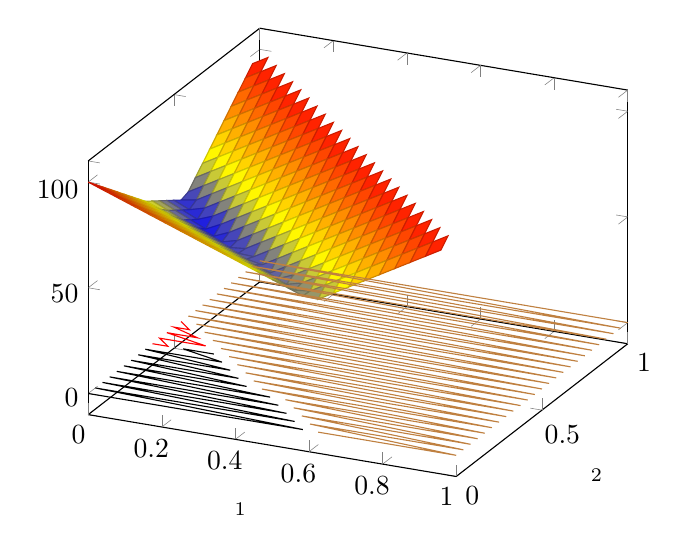
\begin{tikzpicture}
    \begin{axis}[
        xlabel=$\w_1$,
        ylabel=$\w_2$,
        domain=0:1,
        y domain=0:1
      ]

      \addplot3[surf, unbounded coords=jump]{x+y<=1?max(90*(1-x-y) + 12*x + 30*y, 90*(1-x-y) + 13*x + 1*y, 90*(1-x-y) + 10*x + 5*y, 1*(1-x-y) + 100*x + 100*y, 100*(1-x-y) + 37*x + 10*y):NaN};
      \addplot3[mark=none,color=red]{90*(1-x-y) + 12*x + 30*y>=max(90*(1-x-y) + 12*x + 30*y, 90*(1-x-y) + 13*x + 1*y, 90*(1-x-y) + 10*x + 5*y, 1*(1-x-y) + 100*x + 100*y, 100*(1-x-y) + 37*x + 10*y)?0:NaN};
      \addplot3[mark=none,color=green]{90*(1-x-y) + 13*x + 1*y>=max(90*(1-x-y) + 12*x + 30*y, 90*(1-x-y) + 13*x + 1*y, 90*(1-x-y) + 10*x + 5*y, 1*(1-x-y) + 100*x + 100*y, 100*(1-x-y) + 37*x + 10*y)?0:NaN};
      \addplot3[mark=none,color=blue]{90*(1-x-y) + 10*x + 5*y>=max(90*(1-x-y) + 12*x + 30*y, 90*(1-x-y) + 13*x + 1*y, 90*(1-x-y) + 10*x + 5*y, 1*(1-x-y) + 100*x + 100*y, 100*(1-x-y) + 37*x + 10*y)?0:NaN};
      \addplot3[mark=none,color=brown]{1*(1-x-y) + 100*x + 100*y>=max(90*(1-x-y) + 12*x + 30*y, 90*(1-x-y) + 13*x + 1*y, 90*(1-x-y) + 10*x + 5*y, 1*(1-x-y) + 100*x + 100*y, 100*(1-x-y) + 37*x + 10*y)?0:NaN};
      \addplot3[mark=none,color=black]{100*(1-x-y) + 37*x + 10*y>=max(90*(1-x-y) + 12*x + 30*y, 90*(1-x-y) + 13*x + 1*y, 90*(1-x-y) + 10*x + 5*y, 1*(1-x-y) + 100*x + 100*y, 100*(1-x-y) + 37*x + 10*y)?0:NaN};

    \end{axis}
  \end{tikzpicture}

\end{figure}

\end{document}